\documentclass[makesolutionspdf]{esg8022pset}
\begin{preamble}
\usepackage{amsmath}
\usepackage{amssymb}
\usepackage{enumerate}
\usepackage{graphicx}
\usepackage{hyperref}
\usepackage{mathtools}
\usepackage[per-mode=symbol]{siunitx} %If this line is giving you trouble, try replacing per-mode with per
%use inter-unit-separator={}\cdot{} ?
\providecommand{\uvec}[1]{{\hat{\bf{#1}}}}
\usepackage{pgf,tikz}
\usetikzlibrary{arrows}
\usepackage{wasysym}
\usepackage{subfig}
\makeatletter
\newcommand{\interitemtext}[1]{%
  \begin{list}{}
   {\itemindent=0mm\labelsep=0mm
   \labelwidth=0mm\leftmargin=0mm
   \addtolength{\leftmargin}{-\@totalleftmargin}}
    \item #1
  \end{list}
}
\makeatother
\renewcommand{\d}{\,d}
\providecommand{\norm}[1]{\lVert#1\rVert}

\newcommand{\Kgrad}{\left(\hat{x} \frac{\partial}{\partial x} + \hat{y} \frac{\partial}{\partial y} + \hat{z} \frac{\partial}{\partial z}\right)}
\newcommand{\Kdiv}[6]{{#4}\left(\frac{\partial {#1}}{\partial x} {#5} \frac{\partial {#2}}{\partial y} {#6}\frac{\partial #3}{\partial z} \right)}
\newcommand{\KKdiv}[6]{{#4}\left(\frac{\partial}{\partial x}{#1} {#5} \frac{\partial}{\partial y}{#2} {#6}\frac{\partial}{\partial z}{#3} \right)}
\newcommand{\dx}{\frac{\partial}{\partial x}}
\newcommand{\dy}{\frac{\partial}{\partial y}}
\newcommand{\dz}{\frac{\partial}{\partial z}}
\newcommand{\dtheta}{\frac{\partial}{\partial \theta}}
\newcommand{\dr}{\frac{\partial}{\partial r}}

\AtBeginDocument{%
  % Appologies to any future editor on the inconsistencies in TeX code and the unnecessary braces.  I'm aggregating previously typeset problems, and didn't think it worth my time to improve the quality of TeX code in ways that won't make any difference to the typeset material. -Jason Gross (jgross@mit.edu)
}%
\end{preamble}

\classname{Physics 8.022}
\semester{Spring 2011}
\problemsetnumber{8} %Put the problem set number here
\duedate{Tuesday, April 5th at 9 \textsc{pm}}
%\readingassignment{Kleppner and Kolenkow, \emph{An Introduction to Mechanics}, Chapters Seven and Eight}
\problemsettitle{Amp\`{e}re's law, Biot-Savart law}

\begin{document}

\begin{problem}{Long flat conductor}
  A long flat conductor of width $a$ carries a sheet of current $i$ (see
  \autoref{fig:flat}). You are asked to find the magnetic field (direction and
  magnitude) near the center of its flat side and and very close to the
  surface, such that the distance $R$ from the sheet is $R \ll a$.

  \begin{figure}[ht]
    \centering
    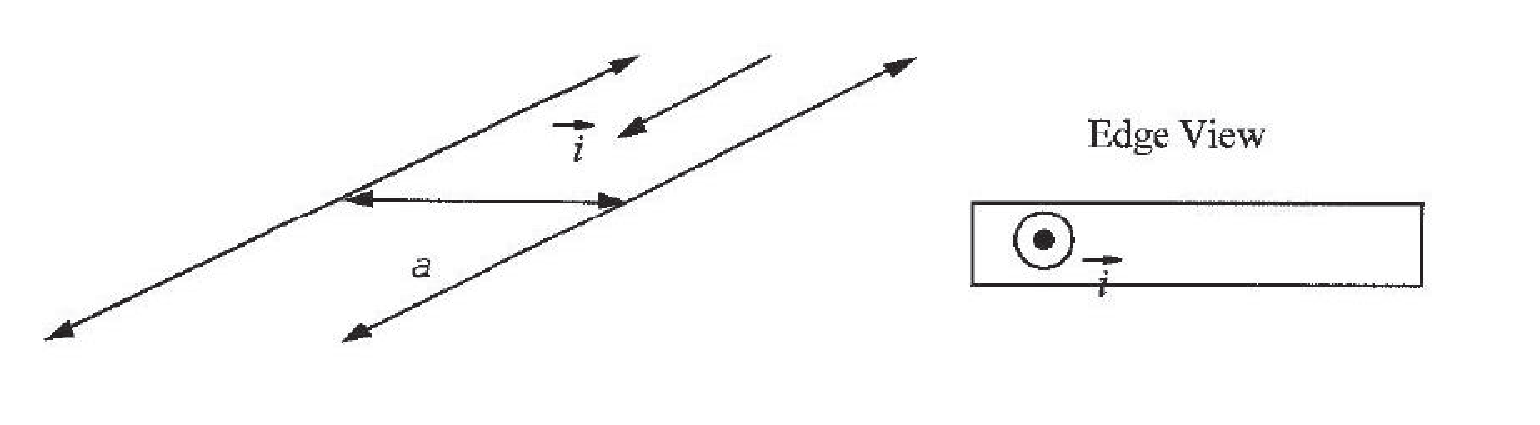
\includegraphics[width = 10cm]{flat_conductor}
    \caption{Flat conductor}
    \label{fig:flat}
  \end{figure}

\end{problem}

\begin{solution}

  \begin{figure}[ht]
    \centering
    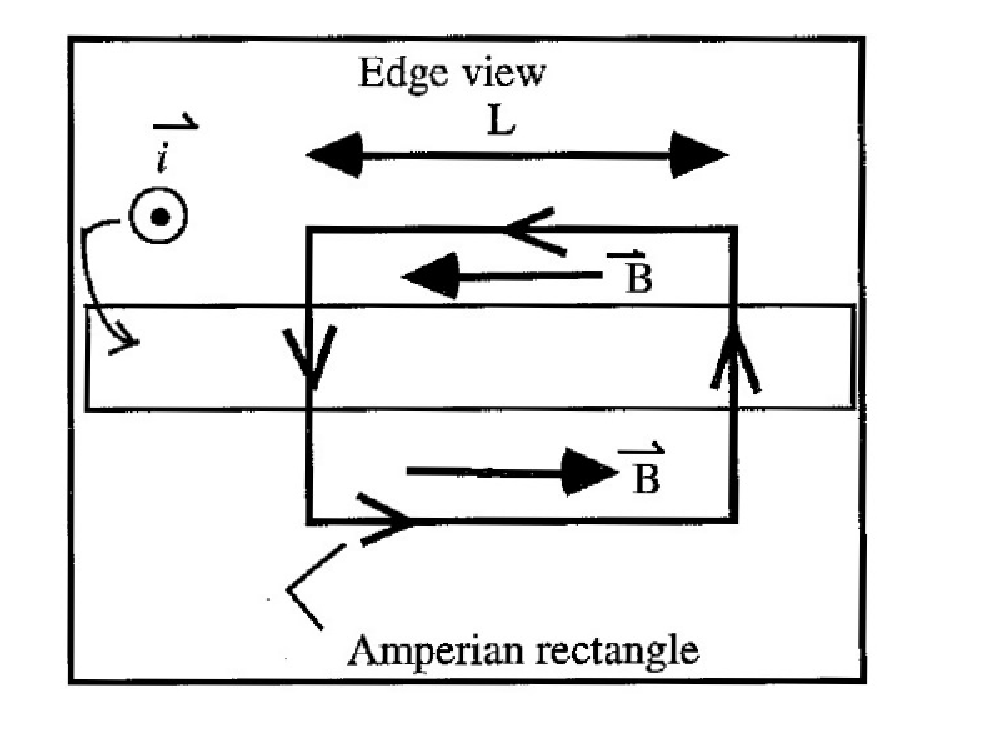
\includegraphics[width = 12cm]{flat_conductor_sol}
    \label{fig:flatsol}
  \end{figure}

  As shown in the figure, above the conductor, $\vec{B}$ points to the left,
  below the conductor, $\vec{B}$  points to the right (the current is pointing
  out of the paper).  Choose an amperian path shown in the plot, since the
  distance $R$ is much smaller than $a$, we have:
  \begin{equation}
    2B \times L = \frac{4 \pi}{c} I_{\text{enc}} = \frac{4 \pi}{c} \frac{L i}{a}
  \end{equation}
  Hence $B=\frac{2 \pi i}{a c}$.
\end{solution}


\begin{problem}{Magnetic field of three wires --- Purcell 6.5}
Three long straight parallel wires are located as shown in the diagram. One wire (B) carries current $2 I$ into the paper;
 each of the others (A and C) carries current $I$ in the opposite direction. What is the strength if the magnetic field at $P_1$
  and $P_{2}$?
  
   \begin{figure}[ht]
    \centering
    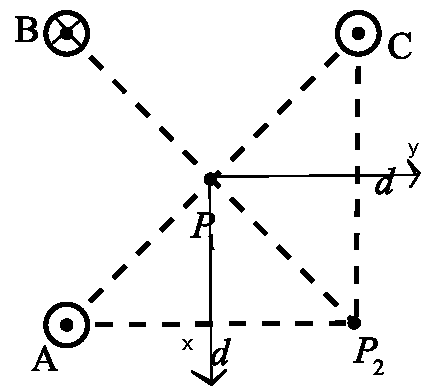
\includegraphics[width = 5cm]{Threewires}
    \label{fig:threewire}
  \end{figure}
  
\end{problem}
\begin{solution}
The field generated by the wires $A$ and $C$ cancel at the point $P_{1}$. Hence, the magnetic field at point $P_{1}$ is same as the magnetic field due to the wire $B$ which is,
$$\vec{B}_{1} = -\frac{2 (2I)}{ c d/\sqrt{2}} \left( \frac{1}{\sqrt{2} } \hat{x}+\frac{1}{\sqrt{2} } \hat{y} \right) = -\frac{4I}{cd} ( \hat{x} +  \hat{y})$$
This field is perpendicular to the line joining $B$ and $P_{1}$ and it points towards $A$.\\
\noindent  The magnetic field due to wire $A$ at point $P_{2}$ is
$$\vec{B}_{2A} =\frac {2 I}{cd}  \hat{y}$$
Similarly, the field due to the wire $C$ is
$$\vec{B}_{2C} = \frac{2 I}{cd}  \hat{x}$$
The contribution of the wire $B$ to the field at point $P_{2}$ is half of its contribution to the field at $P_{1}$: 
$$\vec{B}_{2B} =  -\frac{2I}{cd} ( \hat{x} +  \hat{y)}$$
Hence, the net magnetic field at point $P_{2}$ is zero.
\end{solution}

\begin{problem}{Bent wire revisited}
In class we found the magnetic field at the center of a wire bent through $180^\circ$.
Solve it instead for the wire bent through some arbitrary angle.
\end{problem}

\begin{solution}


   \begin{figure}[ht]
    \centering
    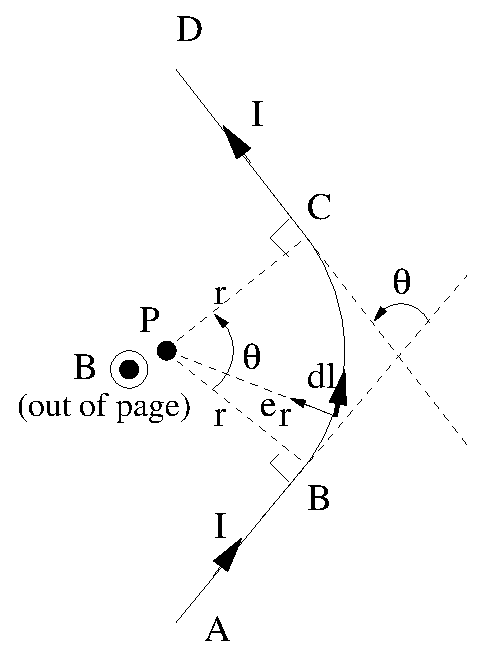
\includegraphics[width = 5cm]{BS1v05}
    \label{fig:bentwire}
  \end{figure}

Refer to Figure \autoref{fig:bentwire}.  To calculate the magnetic
field, we decompose the wire into two semi-infinite long wires AB and
CD and an arc BC of angle $\theta$.  Each part of the wire contribute to $\vec{B}$ in
the same direction, that is normal to and out of the page.  By Ampere's law we
can calculate a magnetic field of a {\sl whole} infinite long wire
$B\times 2\pi r=(4\pi/c)I$, or $B=2I/cr$.   $\vec{B}$ given by the
{\sl half}-infinite long wire AB is just $B_{AB}=(1/2)\times
(2I/cr)=I/cr$.  The same amount is contributed to $\vec{B}$ given by
CD.  For the arc BC,
\begin{equation}
B_{BC}=\int\frac{Idl}{cr^2}=\frac{I\times \theta r}{cr^2}=\frac{\theta I}{cr}\quad\textrm{($\theta$ in radian)}
\end{equation}
So the total magnetic field at point P is 
\begin{equation}
\vec B_P=\frac{(2+\theta)I}{cr}\hat z\;,
\end{equation}
where $\hat z$ points out of the page.

\end{solution}

\begin{problem}{Magnetic field due to a spinning disk}
A flat circular disk with radius $R$ carries a uniform surface charge density
$\sigma$. It rotates with an angular velocity $\omega$ about the $z$-axis. 
Find the magnetic field $\vec{B}(z)$ at any point $z$ along the rotation axis.

   \begin{figure}[ht]
    \centering
    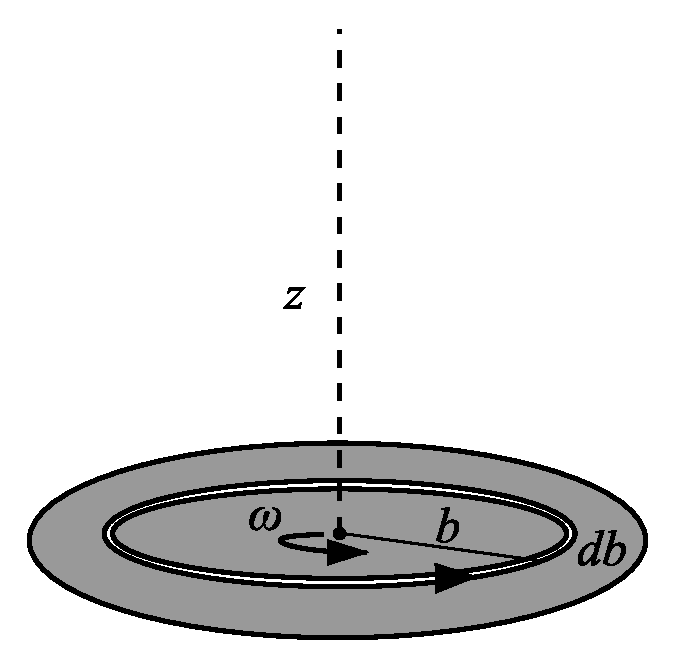
\includegraphics[width = 5cm]{Spinningdisk}
    \label{fig:spinningdisk}
  \end{figure}
  
\end{problem}
\begin{solution}
We treat the spinning disk as a
series of infinitesimal loops for which we already know the field. The
field generated by a loop of radius $b$ is
$$B_z = \frac{2\pi b^2 I}{c(b^2+z^2)^{\frac{3}{2}}}\quad\rightarrow\quad dB_z = \frac{2\pi b^2 dI}{c(b^2+z^2)^{\frac{3}{2}}} \quad dI = \sigma\omega bdb$$
 Integrating over the whole disk we find,
$$B_z = \int_0^R \frac{2\pi b^2 \sigma\omega
b}{c(b^2+z^2)^{\frac{3}{2}}}db =
\frac{2\pi\sigma\omega}{c}\left(\frac{R^2+2z^2}{\sqrt{R^2+z^2}}-2|z|\right)
$$
\end{solution}

\begin{problem}{Coaxial cable}
A long coaxial cable consists of two concentric conductors, as shown in Fig. \autoref{fig:spinningdisk} below.
The inner conductor is a cylinder with radius $a$, and it carries a current $I$ 
uniformly distributed over its cross section. The outer conductor is a cylindrical shell with 
inner radius $b$ and outer radius $c$. It carries a current $I$ that is also uniformly 
distributed over its cross section, and that is opposite in direction to the current of the 
inner conductor.  Calculate the magnetic field $\vec{B}$  and plot the field strength as a function of
the distance from the axis.

   \begin{figure}[ht]
    \centering
    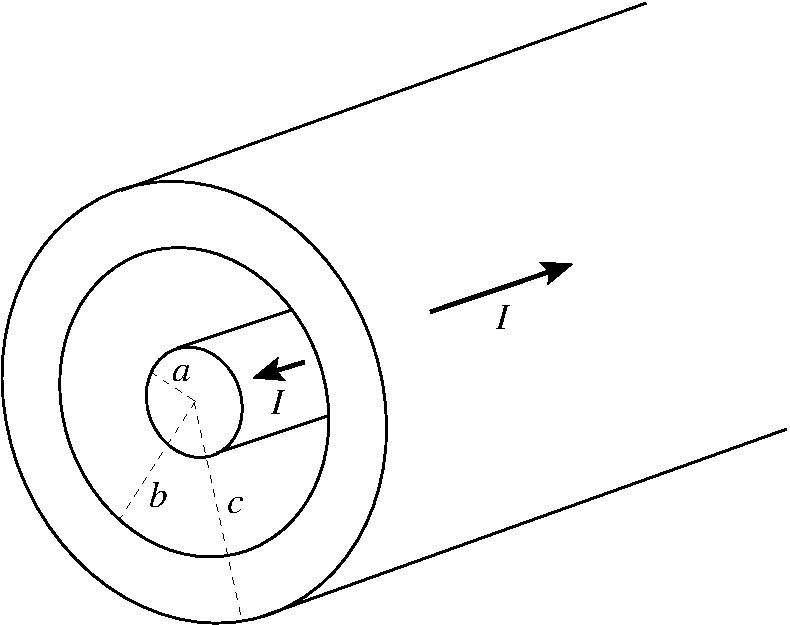
\includegraphics[width = 5cm]{coax}
    \caption{Cross-section of a long coaxial cable.}   
    \label{fig:spinningdisk}
  \end{figure}
\end{problem}

\begin{solution}
We will make use of the cylindrical symmetry and Ampere's law to evaluate the magnetic field everywhere. 
\begin{itemize}
\item In the region $R<a$,
$$2\pi R B = \frac{4\pi}{c} J_1\pi R^2 \implies \vec{B} = \frac{2IR}{ca^2}\hat{\theta}$$
where $J_1$ is the current density in this region and it is given by,
$$J_{1} = {I \over \pi a^{2}}$$
\item
In the region $(b > R > a)$ $$  2\pi R B = \frac{4\pi}{c} J_1\pi a^2
\implies \vec{B} = \frac{2I}{cR}\hat{\theta}$$
\item
In the region $(c > R > b)$, the current density is $J_{3} = I/\pi ( c^2 - b^2 )$. Hence,
 $$2\pi R B = \frac{4\pi}{c} ( I  -
J_3\pi(R^2-b^2)) \implies \vec{B} =
\frac{2I}{cR}\left(\frac{c^2 - R^2}{c^2 -b^2}\right)\hat{\theta}$$
\item
In the region $(d > R > c)$ $$ B.2\pi R = \frac{4\pi}{c} ( I - I) \implies \vec{B} = 0 $$
\end{itemize}
\end{solution}

\begin{problem}{Rectangular Toroidal Solenoid --- Purcell 6.14}

What is the magnetic field inside and outside of the solenoid in figure \autoref{fig:toroid}?

   \begin{figure}[ht]
    \centering
    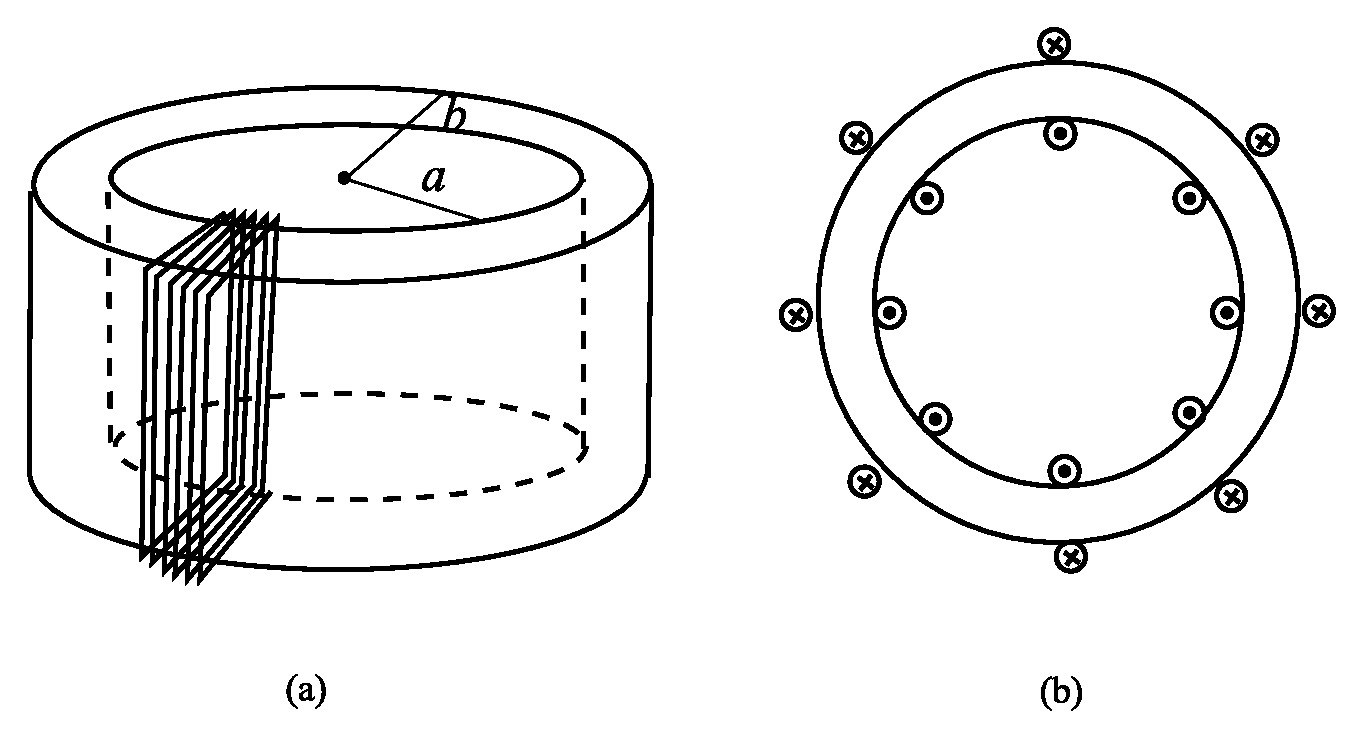
\includegraphics[width = 5cm]{Toroid}  
    \label{fig:toroid}
  \end{figure}

\end{problem}
\begin{solution}
Cylindrical symmetry demands that the magnetic field must be azimuthal everywhere and has only radial dependence.
Note that the current enclosed by a circular
Amperian loop with radius less than the inner radius encloses zero current {\it i.e.}, $I_{enc} = 0$.
A circular Amperian loop with radius greater than the outer radius encloses zero net current ($I_{enc} = NI - NI = 0$). Therefore, the field is zero
everywhere outside the toroid.

The field inside can be calculated using Ampere's
law as follows.
$$\oint \vec{B} \cdot d\vec{s} = \frac{4\pi}{c}I_{enc}  \implies \quad B 2 \pi R
= \frac{4\pi}{c}NI  \implies \quad \vec{B} =
\frac{2NI}{cR}\hat{\theta} $$

\end{solution}

\begin{problem}{Vector potential of a solenoid }
Find the vector
potential $\vec A$ inside and outside of an infinite solenoid of
radius $R$ with $n$ turns per centimeter, each carrying current $I$.
Find the solution for $\vec A$ which is symmetric about the axis of
the solenoid.

{\bf HINT}: You can come up with a {\it very} simple way to compute
$\vec A$ by putting together

\begin{itemize}

\item The magnetic flux, $\Phi_B = \int \vec B\cdot d\vec a$

\item The definition $\vec B = \vec\nabla\times\vec A$

\item Stoke's theorem.
\end{itemize}

\end{problem}
\begin{solution}
What is the magnetic field inside and outside of the solenoid in figure \autoref{fig:toroid}?
   \begin{figure}[ht]
    \centering
    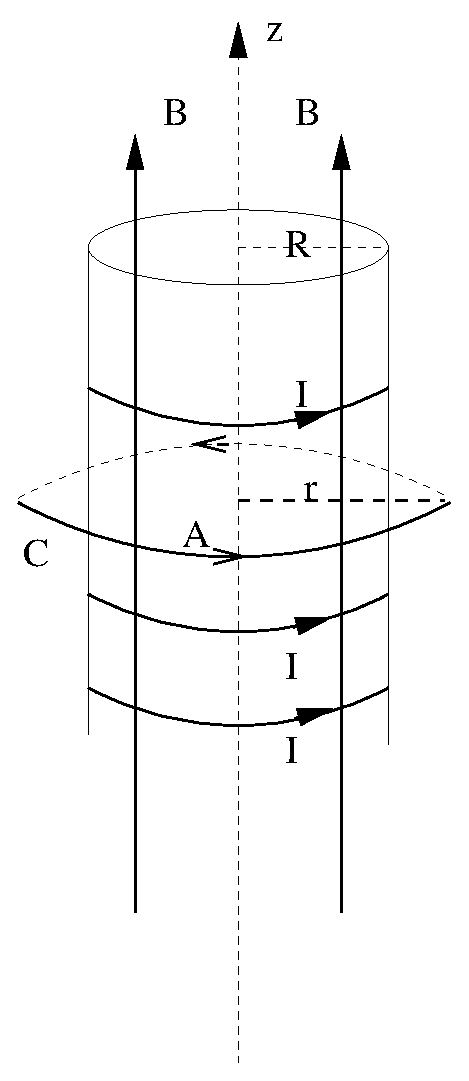
\includegraphics[width = 5cm]{vecpot7}  
    \label{fig:potential}
  \end{figure}
The magnetic field of a infinite solenoid is uniform inside and zero outside them.  By Ampere's law, $Bl=(4\pi/c)nlI$ for
$r<R$ where $l$ is some axial length.  So
\begin{equation}
\vec{B}= \left\{\begin{array}{r@{\quad,\quad}l}
(4\pi/c)nI\hat{z} & r<R\\0 & r>R \end{array} \right.
\end{equation}
The  magnetic flux through a surface area bounded by a
circle $C$ of radius $r$ (see Figure \autoref{fig:potential}) is:
\begin{equation}
\Phi_B = \left\{\begin{array}{r@{\quad,\quad}l}
(4\pi^2/c)nIr^2 & r<R\\ (4\pi^2/c)nIR^2 & r>R 
\end{array} \right.
\end{equation}
  By Stoke's Theorem,

\begin{eqnarray}
\Phi_B &=& \int \vec{B}\cdot d\vec{a}=\int \nabla\times\vec{A}\cdot
d\vec{a}\nonumber\\
&=& \oint \vec{A}\cdot d\vec{l}\nonumber.
\end{eqnarray}

We seek  a solution that is symmetric about the z-axis.  The
simplest one is $\vec{A}=A\hat\phi$, i.e. along the ``circumferential''
direction.
\[ \oint \vec{A}\cdot d\vec{l}\nonumber = A\times 2\pi r.\]
Therefore, 
\begin{equation}
A = \left\{\begin{array}{r@{\quad,\quad}l}
(2\pi/c)nIr & r<R\\ (2\pi/c)nIR^2/r & r>R \end{array} \right.
\end{equation}
You can check  that $\nabla\times \vec{A}=\vec{B}$ in
cylindrical coordinates  both inside and outside.  Note that 
in the exterior $\vec{A}$ is non-zero, even though $\vec{B}$ is zero there.

\end{solution}


\begin{problem}{The Director's Challenge --Extra credit!!!}
Formulate an interesting problem that relates a topic from 8.022  to your intended major or any topic about which you are passionate.
Give references to help future students to understand the context.
Try to give a solution.  Any method, theoretical,  analytical, numerical, experimental, is acceptable. If you can't
 give a full solution, outline partial solutions. Enjoy!
\end{problem}

\end{document}

